\documentclass{loyola-beamer}
\renewcommand{\titlelogo}{logo/luc-rev.svg}
\renewcommand{\slidelogo}{logo/luc.svg}
\usepackage{physics}
\usepackage{graphicx}
\usepackage{hyperref}


\title{Summer Training - ICS399}
\subtitle{Software Engineer at Mawqoot}

\author{Alfaifi, Ammar}
\institute{KFUPM}
\renewcommand{\slidefoot}{Department of Information \& Computer Science}

\begin{document}

\begin{titleframe}{}
	\maketitle
\end{titleframe}

\begin{frame}{Contents}
	\tableofcontents
\end{frame}


% Start of the slides

\section{About Me}

\begin{frame}{About me :)}
  I'm Ammar Alfaifi, senior student. Some work I've done
	\vspace{\baselineskip}

	\begin{itemize}
		\item Double major in Physics and Computer science.
		\item Simulation and physics numerical solutions.
		\item ML and AI models: Weather status predictor. \href{https://github.com/ammar-faifi/Weather\_Status\_Predictor\_From\_Images}{\underline{Repo}}
		\item Worked on many \texttt{djagno} projects, GraphQL/REST API \href{https://Petroly.co/}{\underline{Petroly.co}}
	\end{itemize}

\end{frame}

\begin{titleframe}{Company and Product}
 Info about the company and its main product 
\end{titleframe}

% New slide
\section{Mawqoot and Its Company}

\begin{frame}{Company Info}
  \textbf{Vision:} Our vision is to be at the forefront of pioneering technological advancements. 
  We harness modern technologies to serve various sectors, making them accessible to all
	\vspace{\baselineskip}

  \begin{itemize}
    \item Sanim Information Technology.
    \item located in the Dhahran Techno Valley at KFUPM.
  \end{itemize}
\end{frame}


% New slide
\section{Company's Main Product}

\begin{frame}{Mawqoot}
    \begin{itemize}
        \item Mawqoot presents a cloud-based solution redefining personnel management.
        \item Fusion of mobile apps and a web platform for overseeing attendance, leave, and payroll.
        \item Streamlines operations by replacing paper records and spreadsheets.
        \item Empowers employees with self-service capabilities.
    \end{itemize}
\end{frame}

\begin{frame}{Attendance Management}
    \begin{itemize}
        \item Core: Robust attendance management.
        \item Tracks daily attendance, identifies tardiness, departures, and absences.
        \item App features: Location tracking, biometric verification.
        \item Access to attendance timesheet for corrections.
    \end{itemize}
\end{frame}

\begin{frame}{Compliance and Performance}
    \begin{itemize}
        \item Automated system detects employee infractions, enforces penalties.
        \item Enhances compliance, provides insights for decisions.
    \end{itemize}
\end{frame}

\begin{frame}{Leave and Payroll Management}
    \begin{itemize}
        \item Revolutionizes leave and payroll procedures.
        \item Simplifies leave requests, payroll generation; eliminates paper workflows.
        \item Employees request leave, access annual leave balance.
        \item System deducts leave from salaries, managers approve requests.
        \item Administrators generate detailed payrolls, comprehensive payslips.
    \end{itemize}
\end{frame}

\begin{frame}{Mawqoot inteface}
  \begin{figure}
    \begin{center}
      
\includegraphics[width=0.5\textwidth]{figures/site.png}
    \end{center}
    \caption{The Mawqoot main site, showing the UI.}
  \end{figure}
\end{frame}

\begin{frame}{Mawqoot inteface}
  \begin{figure}
    \begin{center}
      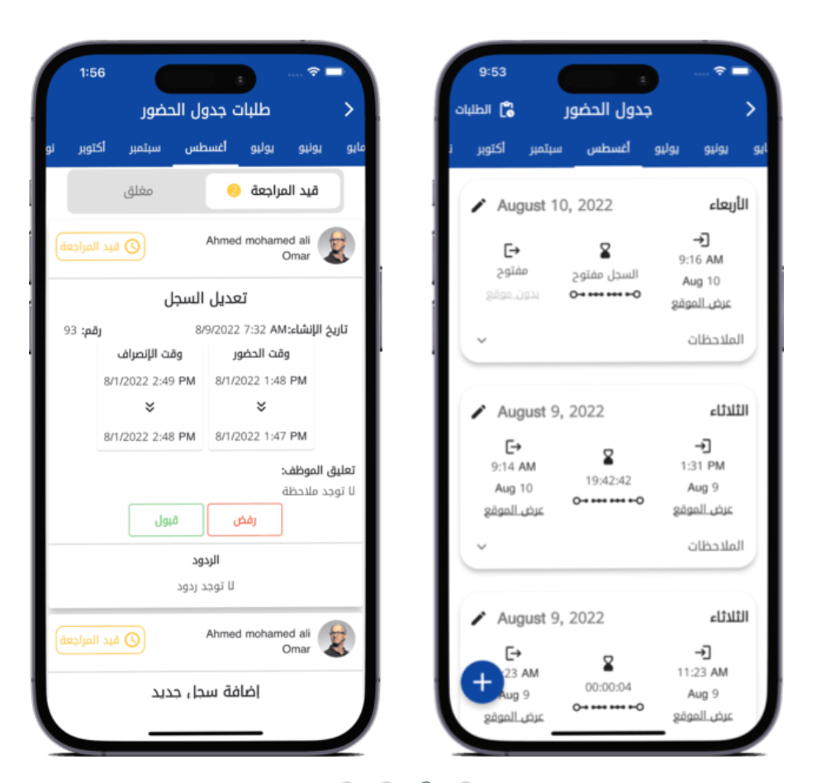
\includegraphics[width=0.45\textwidth]{figures/mobile.png}
    \end{center}
    \caption{A show case for the mobile app.}
  \end{figure}
  
\end{frame}


% ----- Work experience ------- %

\begin{titleframe}{Work Experience}
  Projects and features I worked on during my trainging.
\end{titleframe}

% New Section
\section{Request Petition Feature}

% New Section
\section{Loan Feature}

\begin{frame}{Conclusion}

	In conclusion, coherent states are special types of quantum states which have several
	useful properties and applications. They are widely used in quantum physics, quantum optics,
	and quantum information.

\end{frame}


\begin{titleframe}{Thank you for listening!}

\end{titleframe}

\end{document}
